\documentclass[letterpaper,10pt]{article}

\usepackage{titling}
\usepackage{listings}
\usepackage{url}
\usepackage{setspace}
\usepackage{subfig}
\usepackage{sectsty}
\usepackage{pdfpages}
\usepackage{colortbl}
\usepackage{multirow}
\usepackage{relsize}
\usepackage{amsmath}
\usepackage{fancyvrb}
\usepackage{amsmath,amssymb,amsthm,graphicx,xspace}
\usepackage[titlenotnumbered,noend,noline]{algorithm2e}
\usepackage[compact]{titlesec}
\usepackage{paratype} 
\usepackage[T1]{fontenc}
\usepackage{tikz}
\usetikzlibrary{arrows,automata,shapes,trees,matrix,chains,scopes,positioning,calc}
\tikzstyle{block} = [rectangle, draw, fill=blue!20, 
    text width=2.5em, text centered, rounded corners, minimum height=2em]
\tikzstyle{bw} = [rectangle, draw, fill=blue!20, 
    text width=4em, text centered, rounded corners, minimum height=2em]

\definecolor{namerow}{cmyk}{.40,.40,.40,.40}
\definecolor{namecol}{cmyk}{.40,.40,.40,.40}

\let\LaTeXtitle\title
\renewcommand{\title}[1]{\LaTeXtitle{\textsf{#1}}}


\newcommand{\handout}[5]{
  \noindent
  \begin{center}
  \framebox{
    \vbox{
      \hbox to 5.78in { {\bf ECE254: Operating Systems and Systems Programming } \hfill #2 }
      \vspace{4mm}
      \hbox to 5.78in { {\Large \hfill #4  \hfill} }
      \vspace{2mm}
      \hbox to 5.78in { {\em #3 \hfill} }
    }
  }
  \end{center}
  \vspace*{4mm}
}

\newcommand{\lecture}[3]{\handout{#1}{#2}{#3}{Lecture #1}}
\newcommand{\tuple}[1]{\ensuremath{\left\langle #1 \right\rangle}\xspace}

\addtolength{\oddsidemargin}{-1.000in}
\addtolength{\evensidemargin}{-0.500in}
\addtolength{\textwidth}{2.0in}
\addtolength{\topmargin}{-1.000in}
\addtolength{\textheight}{1.75in}
\addtolength{\parskip}{\baselineskip}
\setlength{\parindent}{0in}
\renewcommand{\baselinestretch}{1.5}
\newcommand{\term}{Spring 2015}

\singlespace


\begin{document}

\lecture{ 29 --- Scheduling in Common Operating Systems }{\term}{Jeff Zarnett}

In this lecture we will examine how real commercial operating systems schedule their processes and threads. We will examine UNIX, Linux, and finally Windows scheduling. We will see what approaches are used and what is interesting or novel about them.

\subsection*{Traditional UNIX}

The traditional UNIX scheduling is really ancient; as in System V R3 and BSD 4.3. It was replaced in SVR4 (which had some real-time support). The information about the traditional UNIX scheduler comes primarily from~\cite{osi}

The routine is a multilevel feedback system using Round Robin within each of the priority queues. Time slicing is implemented and the default time slice is a (very long) 1 second. So if a process does not block or complete within 1~s, then it will be preempted. Priority is based on the process type as well as the execution history.

Processor utilization for a process $j$ is calculated for an interval $i$ by the following formula:

\begin{center}
$CPU_{j}(i) = \dfrac{CPU_{j}(i - 1)}{2}$
\end{center}

And the priority is for process $j$ at interval $i$ is calculated by the formula:

\begin{center}
$P_{j}(i) = B_{j} + \dfrac{CPU_{j}}{2} + N_{j}$
\end{center}

where $B_{j}$ is the base priority of process $j$ and $N_{j}$ is the ``nice'' value of process $j$. The ``nice'' value is a UNIX way to allow a user to voluntarily reduce the priority of a process to be ``nice'' to other users (but honestly, who uses this?)~\cite{mos}. Actually, the answer to that question is: system administrators. An admin can ``re-nice'' a process and make it somewhat nicer than it would otherwise be.

The $CPU$ and $N$ components of the equation are restricted prevent a process from migrating outside of its assigned category. A process is assigned to a given category based on what kind of process it is. To put it in simple terms, the OS puts its own needs first and tries to make the best use of resources it can. From highest to lowest priority, the categories are:

\begin{enumerate}
	\item Swapper (move processes to and from disk)
	\item Block I/O device control (e.g., disk)
	\item File manipulation
	\item Character I/O device control (e.g., keyboard)
	\item User processes
\end{enumerate}

Yes, unfortunately, user processes get piled at the bottom of the list. The use of the hierarchy should provide for efficient use of I/O devices and tends to penalize processor-bound processes at the expense of I/O bound processes. This is beneficial, because CPU-bound processes should be able to carry on executing when an I/O-bound process waits for the I/O operation to complete, but when an I/O operation is finished, we would like to start the next I/O operation so the I/O device is not waiting. This strategy is reasonably effective for a general-purpose, time-sharing operating system.

\subsection*{Linux}
Linux has two scheduling modes: Real-Time and Non-Real-Time (or perhaps we should call that the ``normal'' one). It is not necessary to use the real-time scheduler, strictly speaking, and if the real-time scheduler is used, the system can still have non-real-time threads which will be scheduled according to the normal scheduler routine.

\subsubsection*{Linux Real-Time Scheduler}

The Linux scheduler operates based on \textit{scheduling classes}, which are very much like the categories above. There are three classes into which priorities can be assigned~\cite{osi}:

\begin{itemize}
	\item \texttt{SCHED\_FIFO}: First-In, First-Out Real-Time threads
	\item \texttt{SCHED\_RR}: Round-Robin Real-Time threads
	\item \texttt{SCHED\_OTHER}: Other (non-real-time) threads.
\end{itemize}

In each class, threads may have different priorities relative to one another. Lower numbers indicate higher priorities. Real-time priorities are in the range [0-99] and the other priorities are [100-139].

The rules for \texttt{SCHED\_FIFO} are as follows~\cite{osi}:

\begin{enumerate}
	\item The system will only interrupt a FIFO thread if one of the following is true:
	\begin{enumerate}
		\item Another FIFO thread of higher priority becomes read.
		\item The current FIFO thread gets blocked (e.g., on I/O).
		\item The current FIFO thread yields the CPU with \texttt{sched\_yield}.
	\end{enumerate}
	\item If a FIFO thread is interrupted, it is placed in the queue associated with its priority.
	\item If a FIFO thread becomes ready and that thread has higher priority than the currently-executing thread, the currently-executing thread is preempted in favour of the highest priority ready FIFO thread. If two or more threads are at the highest priority, the one that has been waiting the longest is chosen.
\end{enumerate}

The policy is the same for Round-Robin real-time scheduling, except time slicing is implemented. So if a Round-Robin thread has executed for a full time slice it is suspended and the scheduler will select a real-time thread of equal or higher priority (which could certainly be the same thread, but is not necessarily). The difference is illustrated in the diagram below:

\begin{center}
	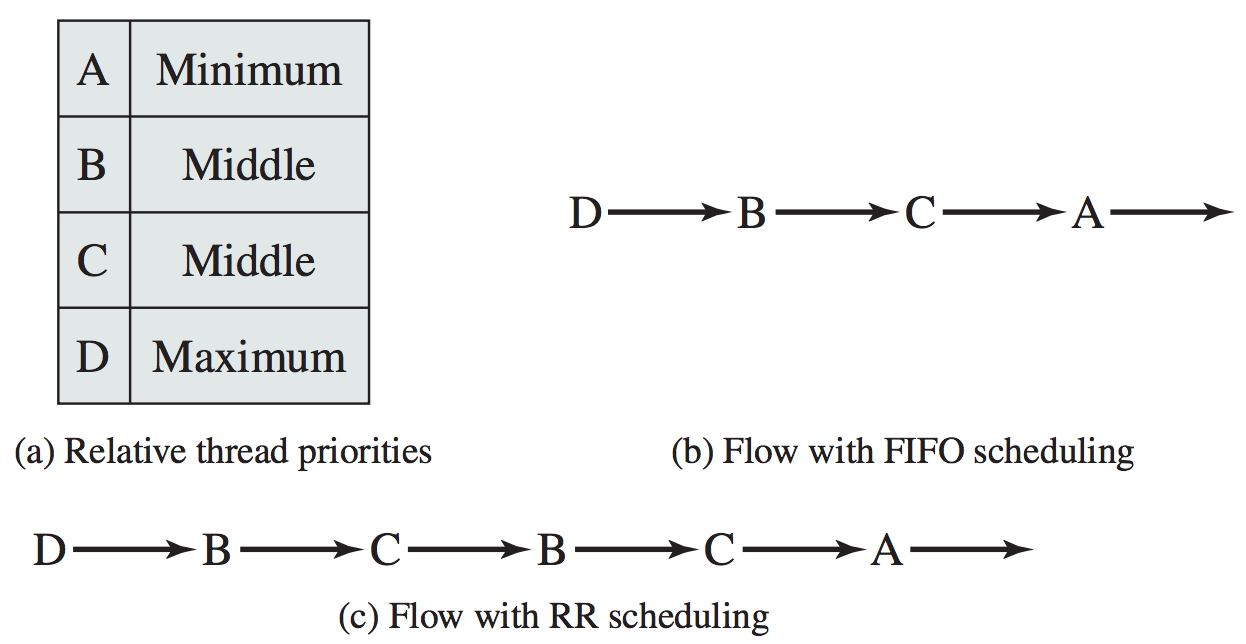
\includegraphics[width=0.55\textwidth]{images/linux-rts.png}\\
	Real-Time scheduling in Linux comparing FIFO to Round-Robin (RR)~\cite{osi}.
\end{center}

One of the threads in the \texttt{SCHED\_OTHER} category can execute only if there are no threads in the Round-Robin or FIFO queues that are ready at the moment.

\subsubsection*{Linux Non-Real-Time Schedulers}
In Linux 2.4 and earlier (shockingly late, now that I think of it), the Linux kernel used something like the traditional algorithm. Then they introduced a scheduling algorithm that was commonly called the $O(1)$ scheduler, because it executed in constant ($O(1)$) under all circumstances. This was a big improvement over the previous scheduling algorithm which ran in $O(n)$ time. It also worked a lot better for SMP systems, because it introduced processor affinity and load balancing. Since version 2.6.23 of the kernel, however, a new scheduling algorithm has replaced the $O(1)$ scheduler; it is called the \textit{Completely Fair Scheduler} (CFS).

Let us start by looking at the $O(1)$ scheduler. The traditional UNIX scheduler fell down on a couple of fronts: it was not very good at handling very large numbers of processes; it was an $O(n)$ algorithm, so its performance got worse as more processes appeared in the system. It also had significant difficulty with SMP systems due to its design, notably~\cite{osi}:

\begin{enumerate}
	\item A single run queue;
	\item A single run queue lock; and
	\item An inability to pre-empt running processes.
\end{enumerate}

The single run queue means a task can and will be scheduled on any processor (good for load balancing), but there is no implementation of processor affinity. Thus, a task running on CPU-0 could be easily reassigned to CPU-1 resulting in lots of cache misses.

The single run queue lock means there is one mutual exclusion construct protecting manipulation of the run queue. Thus, when one processor wants to modify it (enqueueing or dequeueing a task, for example), all other processors have to wait until it is unlocked (which can take non-trivial time as an $O(n)$ operation for sufficiently large values of $n$). Thus, processors may be waiting for something to do.

Finally, pre-emption was not possible; lower priority tasks would continue to execute while higher priority tasks were waiting. Only something getting blocked, a time slice expiration, or an interrupt might cause the scheduler to re-evaluate what process should run next.

The kernel would maintain two data structures for the processor in the system~\cite{osi}:

\begin{verbatim}
struct prio_array {
  int nr_active; /* number of tasks in this array */
  unsigned long bitmap[BITMAP_SIZE]; /* priority bitmap */
  struct list_head queue[MAX_PRIO]; /* priority queues */
}
\end{verbatim}

There is one queue for each priority level, and \texttt{MAX\_PRIO} (140) is both the highest priority and the number of queues. The bitmap array is of a size to provide one bit per priority level, so with 140 levels and 32 bit words, \texttt{BITMAP\_SIZE} is 5. The purpose of the bitmap is to indicate which queues are empty. There is an active queue structure as well as an expired queue structure.

Initially, there are no tasks in any queues and all the bits in the bitmap are zero. If a process is created and enters the ready queue, it is put in the queue corresponding to its priority value. If that queue was previously empty, then its bit in the bitmap is set to 1 to indicate that queue is no longer empty. See the diagram below:

\begin{center}
	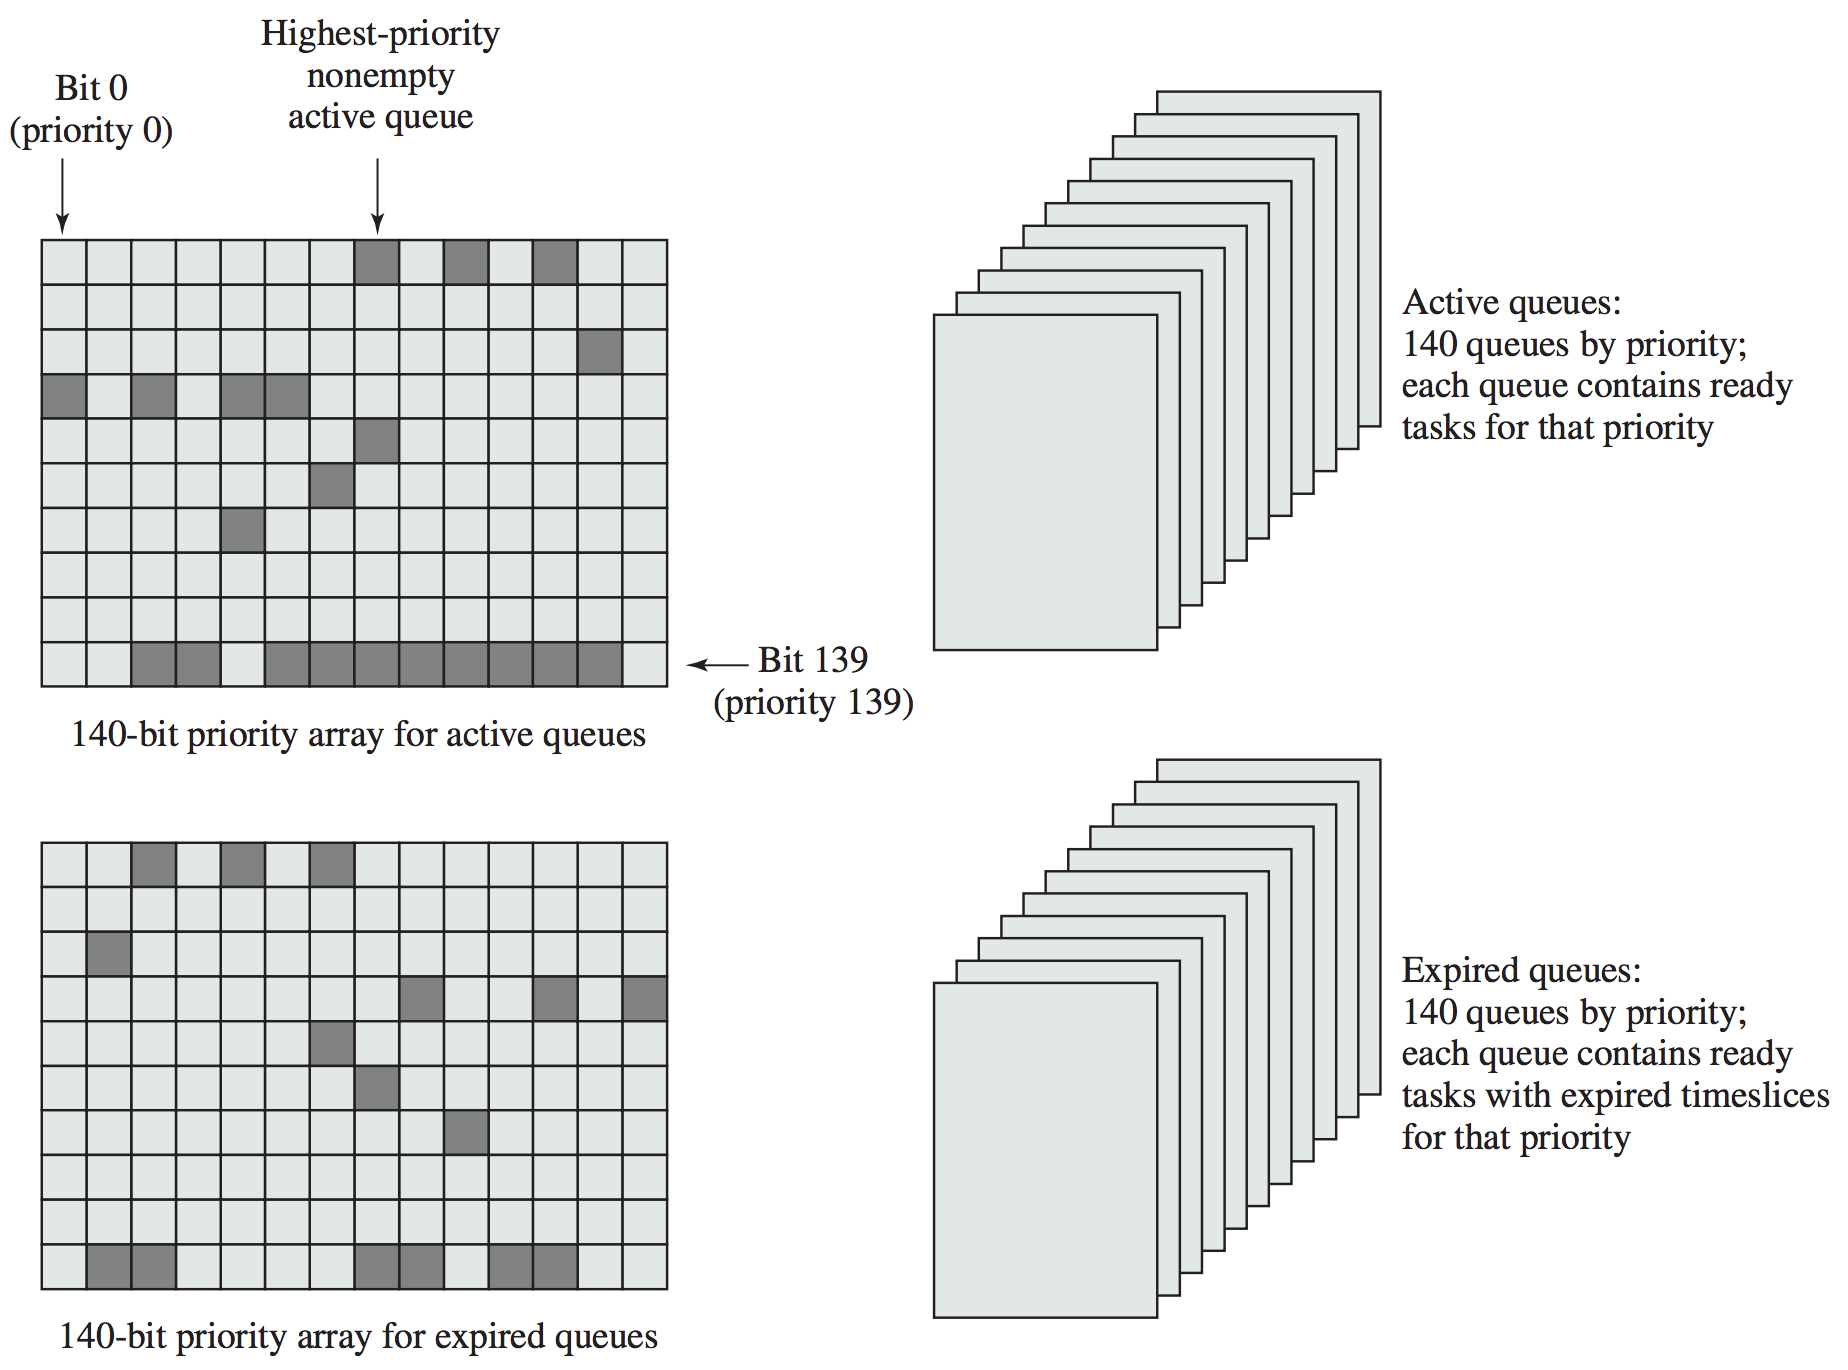
\includegraphics[width=0.75\textwidth]{images/linux-o1-struct.png}\\
	Linux $O(1)$ scheduler internal structures~\cite{osi}.
\end{center}

If a process does not complete its full time slice before it is preempted, then it goes back in the ready queue. If it does run to the end of the time slice, it is placed in the expired queue instead. All scheduling takes place from the active queues. The highest priority queue is chosen; if there are multiple tasks in that queue, they are scheduled in Round-Robin fashion. This continues until the active queue structure is empty. When that happens, the active and expired queues change places, and execution (scheduling) continues~\cite{osi}.

Part of the difficulty with the $O(1)$ scheduler is that it does not provide very good performance for interactive processes, notably the ones you work with on your desktop computer. Given that the Linux folks always claim that this year or next year is ``the year of the Linux desktop'' (... still waiting for that) a new scheduler was needed

The CFS, written by Ingo Moln\'ar, is not $O(1)$, unfortunately. It uses a red-black tree to model the ready queue, where processes are inserted based on a linear ordering of execution time. The leftmost node in this tree is therefore the task that has spent the least amount of time executing and that is what will be scheduled next. Because a red-black tree remains balanced, the time to access the leftmost root node will be $O($ln$(n))$, though caching could be used to make access to the next task faster. If a task gets blocked it will not end up in the queue again, but if it reaches the end of a timeslice or gets preempted, then it will be inserted into the tree with its updated execution time, which is very likely not the same place it was taken from (which might require rebalancing the tree (a $O($ln$(n))$ operation)~\cite{mte241}.

\begin{center}
	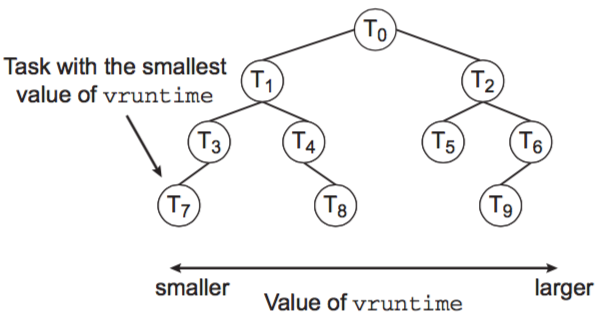
\includegraphics[width=0.5\textwidth]{images/cfs.png}\\
	The Completely Fair Scheduler's red-black tree structure of ready tasks~\cite{osc}.
\end{center}




\subsection*{Windows}

\bibliographystyle{alpha}
\bibliography{254}


\end{document}